\chapter{Diseño}

\noindent

Ya que se ha identificado el problema, su contexto y se ha delimitado los
requerimientos funcionales y restricciones que debe satisfacer la solución se
pasará a definir el diseño de ésta así como las posibles alternativas.

\section{Elección de algoritmo}

El principal reto en la implementación del jugador artificial es que el juego de
dominó es de información imperfecta. Existen dos alternativas principales de
algoritmos que pueden utilizarse en este tipo de juegos.

En primer lugar, existen algoritmos de aprendizaje por refuerzo que han sido
utilizados exitosamente en juegos con incertidumbre e información escondida. El
algoritmo de \textit{Counterfactual Regret Minimization} ha sido utilizado para
crear jugadores de póker. Dicho algoritmo utiliza un enfoque iterativo en el que
se busca aproximar una función que para cada estado del juego defina una acción
óptima.

Por otro lado, existe el algoritmo Perfect Information Monte Carlo (PIMC). En
este algoritmo se busca transformar el juego de información imperfecta en un
conjunto de juegos de información perfecta congruentes con el estado actual del
juego. El conjunto es una muestra aleatoria de los posibles escenarios en los
que el jugador se puede encontrar. En cada uno de estos escenarios se realiza
búsqueda en árbol y al final se toma la acción que en el mayor número de
escenarios llevó a una victoria.

Se considera que PIMC muestra una ventaja sobre la primera alternativa por su
simpleza y facilidad de implementación. Así mismo, permite aprovechar la
experiencia previa que el desarrollador ha tenido implementando jugadores
basados en búsqueda en árbol. Dadas las restricciones del desarrollo, se llegó a
la conclusión que PIMC sería la mejor alternativa para los fines de este
trabajo.

\section{Arquitectura}

El programa consta de los siguientes módulos:

\begin{enumerate}
   \item Análisis del tablero y jugadas predefinidas
   \item Muestreo de fichas desconocidas (\textit{Determinization})
   \item Búsqueda en árbol de juego con información perfecta
\end{enumerate}


\begin{figure}[ht]
   \begin{center}
      \hbox{\hspace{-5em} 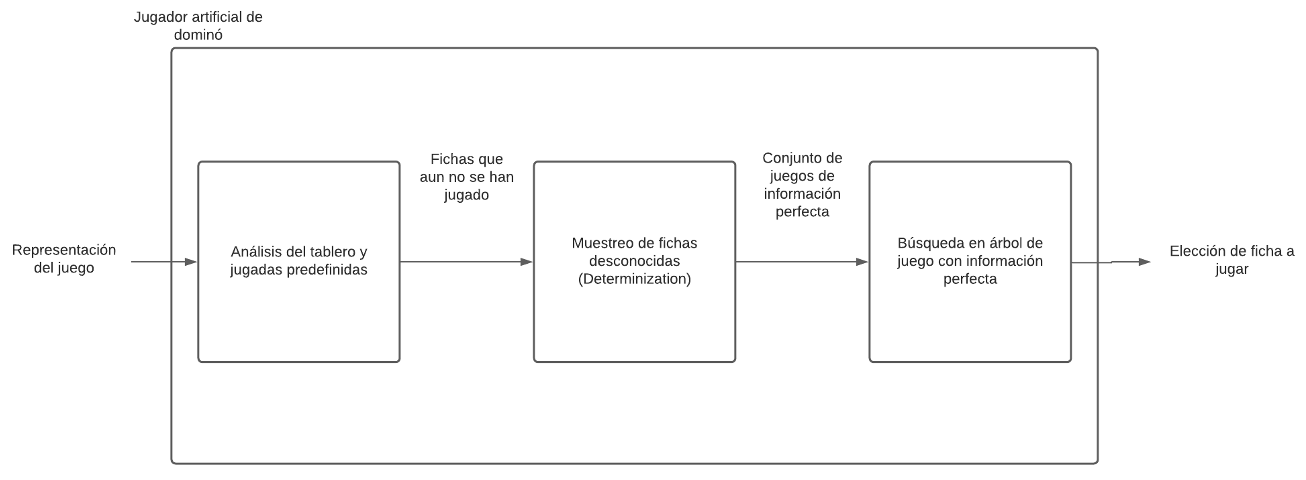
\includegraphics[scale=0.75]{arquitectura.png}}
      \caption{Diagrama de bloques del sistema. El sistema se descompone en tres módulos internos}
      \label{ARQ}
   \end{center}
\end{figure}
El sistema recibe la representación del estado actual del juego externamente.
Cada módulo procesa su entrada y tiene como salida la entrada del siguiente
módulo. La salida del último módulo es la respuesta final del sistema completo.

\section{Análisis de tablero y jugadas predefinidas}

En la primera etapa del sistema, se realiza un análisis del estado del juego que
se recibe como parámetro. En este análisis se busca extraer información
necesaria para el muestreo de la siguiente etapa, así como determinar si existe
una jugada predefinida para el estado actual del juego.

Las circunstancias para utilizar una jugada predeterminada son dos. La primera
es si sólo se tiene una jugada posible, en cuyo caso se realiza dicha jugada sin
iniciar el proceso costoso de búsqueda. La segunda es en el primer turno del
juego, en donde puede ser deseable incorporar conocimiento experto del dominio
para elegir una acción cuando no se cuenta con suficiente información para que
el sistema calcule una jugada efectiva en el límite de tiempo establecido.

Si existe una jugada predefinida se omitirá la ejecución de los demás módulos y
la jugada será la salida del sistema. En otro caso, a partir de la historia del
juego se calcularán las fichas que aun no han sido tiradas y el número de fichas
que tiene cada jugador. Este resultado se pasará al siguiente módulo.

En esta primera versión del sistema sólo implementaremos el caso en que existe
una única jugada posible. Dejamos como linea de investigación para futuras
versiones el incluir conocimiento experto para elegir la primer jugada.

\section{Muestreo de fichas desconocidas}

Siguiendo el algoritmo de PIMC, es necesario generar un conjunto de posibles
escenarios en los que se puede encontrar el jugador. En este caso, los
escenarios se diferencian por las fichas que poseen los otros jugadores. Ya que
se cuenta con el conjunto de fichas que aun no se han jugado, se puede simular
el proceso de repartir las fichas aleatoriamente a los otros jugadores y así
generar los escenarios. Un escenario se conforma de un arreglo en donde se
guardan las fichas que se le repartieron aleatoriamente a cada jugador.

El número de simulaciones que se realizan es un parámetro del sistema que
impacta su comportamiento en dos formas. Entre más simulaciones se realizan,
aumenta el tiempo de ejecución. Entre menos simulaciones, el sistema toma en
cuenta menos escenarios y el desempeño del jugador empeora.

Al final, se recopilan los distintos escenarios en un arreglo y se pasan al
siguiente módulo.

\section{Búsqueda en árbol de juego con información perfecta}

Una vez que se ha transformado el juego en un conjunto de escenarios en los que
se conocen las fichas de los oponentes, es posible calcular una acción óptima
para cada uno de los escenarios. La ficha que el jugador artificial tirará será
aquella que en el mayor número de escenarios fue óptima.

Para hacer el cálculo de la jugada óptima hay distintas
alternativas.\textit{Negamax}, \textit{Alpha-Beta Prunning} y \textit{Monte
   Carlo Tree Search} (MCTS) son los principales candidatos para realizar búsqueda
en árbol de juego con información perfecta

Se eligió el algoritmo MCTS debido a dos características que no comparte con las
dos primeras opciones. En primer lugar, es posible correr el algoritmo sin
necesidad de una heurística, es decir, de una función que estime la utilidad de
un estado del juego. En segundo lugar, MCTS es un algoritmo \textit{anytime}, lo
que significa que la ejecución puede detenerse en un intervalo arbitrario de
tiempo y el algoritmo regresará la mejor jugada que ha encontrado hasta ese
momento.

La segunda propiedad es particularmente apropiada para este sistema ya que
permite controlar el tiempo de ejecución total modificando el tiempo que se
invierte en calcular la acción óptima en cada uno de los escenarios.

\section{Estándares utilizados}

Como parte de la API que el sistema expondrá para ser integrado con otras
plataformas se decidió que la comunicación de información se haga con el
estándar JSON (ECMA-404) debido a su flexibilidad y facilidad de uso. Asimismo,
se utilizará el estándar PEP8 que define una guía de estilo y mejores prácticas
para escribir código en Python.

Conforme a las restricciones planteadas en el análisis del problema, el jugador
debe ser ejecutable en el sistema operativo Ubuntu, el cual sigue el estándar
POSIX.
% \newpage

% \section{Regresión lineal múltiple}

% \subsection{Modelo y resultados}

% \noindent Ulteriormente, se corrió una regresión lineal múltiple en la que la variable dependiente es la innovación y las variables independientes son los cuatro índices construidos: 

% \begin{equation}
%    Y = \beta_{0} + \beta_{1} X_{i1} + \beta_{2} X_{i2} + \beta_{3} X_{i3} + \beta_{4} X_{i4} +\varepsilon, \label{1}
% \end{equation}

% Para escribir ecuaciones

% \begin{table}[H]
% \centering
% \caption{Resultados del modelo econométrico}
% \label{REG}
% \begin{tabular}{|ccccc|}
%   \hline
%  & Estimador & Desv. est. & Valor $t$ & Pr($>|t|$) \\ 
%   \hline
%   $\alpha$ & x & x & x & x \\ 
%   CI & x & x & x & x \\ 
%   IS & x & x & x & x \\ 
%   IR & x & x & x & x \\ 
%   PT & x & x & x & x \\ 
%    \hline
% \multicolumn{5}{|c|}{Error est. de res. = x con x gr. de libertad}
%     \\
%     \multicolumn{5}{|c|}{$R^2$ = x y $\bar{R}^2$ = x}
%  \\
%  \multicolumn{5}{|c|}{Estadístico $F$ = x, con un valor $p$ = x }
%       \\
% \hline
% \end{tabular}

% \end{table}
